 \documentclass[notitlepage]{article}
\usepackage[left=1in, right=1in, top=1in, bottom=1in]{geometry}
\usepackage{subcaption}
\usepackage{graphicx}
\usepackage{natbib}
\usepackage{titling}
\usepackage{lipsum}
\usepackage{amsmath,amssymb}

\pretitle{\begin{center}\Huge\bfseries}
\posttitle{\par\end{center}\vskip 0.5em}
\preauthor{\begin{center}\Large\ttfamily}
\postauthor{\end{center}}
\predate{\par\large\centering}
\postdate{\par}

\title{Lightlane contribution to flux variability}

\author{Jens Tandstad}
\date{\today} 
\begin{document}

\maketitle
\thispagestyle{empty}

\begin{abstract}
Assuming quantized spacetime, Weyl constrains limit the freedom of how information can propagate across the grid. A class of Cellular Automata called Serpentines allows us to circumvent this constraint, but the trade-off is that the constraints lead to a flux variability contribtion separate from the poissonian noise expected from a coninuum model of spacetime. It is possible that this flux variability is detectable in data from space telescopes. The conjecture therefore can act as a stronger no-go theorem for digital physics theories, than that presented by \cite{FritzNoGo}. This paper converts the intution presented in  The Lightlane Conjecture \citep{RhadamantysA2} into a three dimensional analogue and simulate flux variability using Python.
\end{abstract}

\section{Introduction}
In modern physics and cosmology, the equations that we use to predict light transport and wave propagation are continuous, and assume infinite directional freedom for the photon (i.e the path integral is infinite). This allows for analytical solutions. However, it can be difficult to distinguish between finite, high resolution quantized models and their completely continuous approximations. In "Quantized directional freedom or the Lightlane Conjecture" \cite{RhadamantysA2}, I explore a Cellular Automata model of photons, and take advantage of constrains on what such structures can and cannot possibly do. This line of reasoning has been theoretically developed been by David Deutch and Chiara Moretti \cite{DeutchMoretti}, \cite{MorettiVedral} into a framework called Constructor theory, which allows studying the aggregate effects of constrains under quantization.  I show that under assumptions that light obey Cellular Automata constraints, there must be corresponding constraints on directional freedom. Specifically, the set of possible paths extending from a given starting point is related to the size of the propagation program the photon is carrying.

The basis for exploring this connection is the possibility that certain discrete interpretations of quantum mechanics, such the Cellular Automata interpretation of Quantum Mechanics \cite{hooft2014cellular} by Nobel price in Physics laureate Gerard t'Hooft requires that any physical phenomenon that is not space itself must obey constraints that apply to Cellular Automata propagating across a quantized manifold lattice. The bold and fascinating Wolfram Physics project \cite{Wolfram2020} is a different but related approach, studying the evolution of graph structures under substitution rules, some of them producing lattices that could possibly be a model of a quantized spacetime. Both approaches belong to a class of digital quantum interpretations, which  preclude the existence of continuous spacetime, and assume quantized space-time at the Planck scale - or below.

Such interpretations of quantum mechanics are commonly seen as unfalsifiable, because they  make no predictions separate from quantum mechanics. This is logical because they are interpretations, or at best reformulations of quantum mechanics, using information theory. The surprising discreteness of Quantum Mechanics could be fundamental, and the connection to information theory is quite obvious from Heisenbergs matrix formulation of Quantum Mechanics. 


\section{Summary of the Lightlane Conjecture}
There is a possibility that when following a strictly information theoretic approach such Constructor Theory, we can be able to derive constraints on possible and impossible behaviour of objects that exist under such an interpretation. Then, from these constraints we can derive constraints on the aggregate behaviour, which in theory can be detectable as macroscopic phenomena. This provides a way to make contact between this class of quantum foundations and observables. 

The conjecture connects the digital constrains from the Cellular Automata and quantized spacetime constraints to flux variability and blurriness in the data from space telescopes. This is done by quantizing the directional freedom of the photon by assuming it to be a Cellular Automaton, constrained by the Weyl constrains of the quantized spacetime lattice. 

\subsection{Serpentine class TCA}
A class of information structures inspired by the Turing Machine are able to achieve arbitrary directional freedom by increasing the size of it's propagation program. This connect the amount of \textbf{Effective Directional Information} $EDI$, a metric on the amount of information carried by within the photon, to a flux variance contribution $\sigma_L^2$. As the constrains are derived from the interpretation axioms, this might allow for connecting a class of Quantum interpretations of QM with experimental data. This effectively makes the conjecture a no-go theorem for a class of Quantum Foundation theories that relies on Cellular Automata, and therefore must obey Cellular Automata constraints. In the unlikely case that it's novel predictions are verified it could provide a way to probe into sub-quantum mechanics, as well as possibly a new approach to do cosmic distance estimates, taking flux variability and blurriness as parameters. A more likely outcome is that the theory simply constrains the viability of the Serpentine class as a model for the photon. In this paper we convert the intuition from \citep{RhadamantysA2} into a 3D counterpart, and make some crude predictions about flux variability from starlight.

\begin{figure}[!ht]
  \centering
 \includegraphics[width=0.9\textwidth, trim={0cm 0cm 0cm 0cm},clip]{Illustrations/Fig1Serpentine.pdf}
  \caption{M5 Serpentine : Example of Serpentine Class TCA. The instructions are looped, realizing a vector. The precision of the vector depends on the length of the tape.}
      \label{fig:serpentine}
\end{figure}

The metaphysical arguments for exploring such digital constrains is laid out in the Lightlanes Conjecture \cite{RhadamantysA2}, which also discusses past work on digital physics and propagation across crystal lattices. The resulting theory is simple and easy to understand once you accept the motivation. To summarize the paper, assume that all particles, including photons are Cellular Automata that live on an N dimensional grid. Because an excitation of a grid cell is confined to a single cell, it follows from Weyls tile argument that nothing can be in-between cells. The movement of the Cellular Automaton therefore must obey Weyl constraints on propagation. Please see  to Jean Paul Van Bendegems excellent exposition in the Stanford Encyclopedia for a deeper study.  \cite{stanford-geometry-finitism}. 

An effect pertaining to all crystal structures is that the grid limits possible orientations of the Cellular Automata. In regular square crystal in $\mathbb{Z}^n$ to $2^{2n}$, available orientation are $2^n$ orthogonal rotations over  $2^n$ reflections. If space is three dimensional, then only 8 possible directions of propagation through space is possible. Clearly, light can move more in more directions than that. This suggests that directional freedom is not quantized. 

\begin{figure}
\centering
{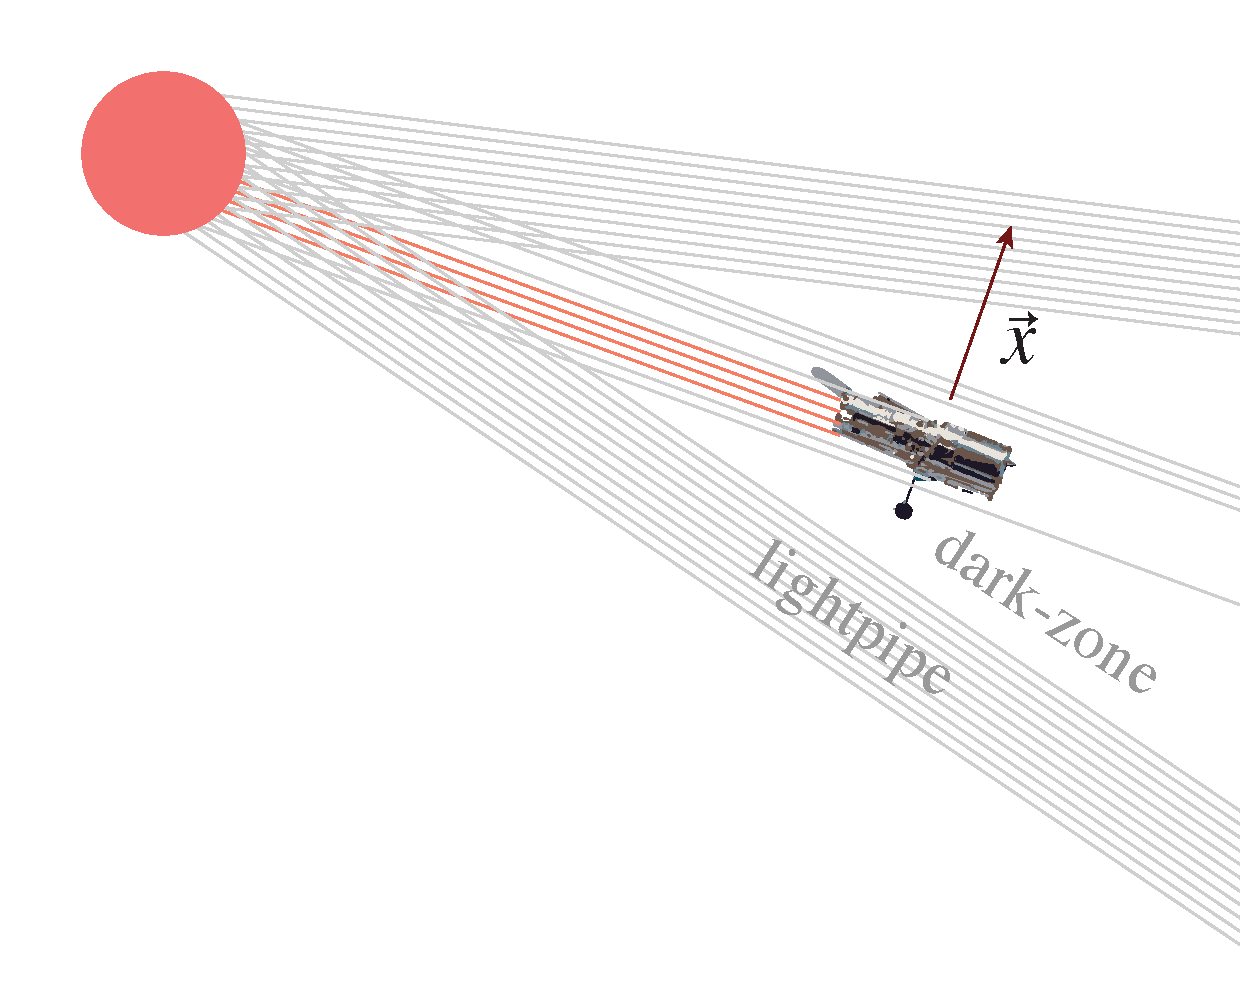
\includegraphics[width=0.7\textwidth, trim={0cm 0cm 0cm 0cm},clip]{illustrations/Hubble.pdf}}
%\subcaptionbox{$ 2r =\sqrt{2}L$  \label{xystion-simple-grid-ratio}}
\caption{Illustration of telescope moving in and out of aggregate dark-zone at speed given by vector $\vec{x} $ per unit of time $t$.  }\label{hubbleDarkZone}
\end{figure}

However, Cellular Automata are diverse and powerful structures. The Serpentine class of TCA, exemplified by the M5 \ref{fig:serpentine}, is \textbf{characterized} by having \textbf{arbitrary directional freedom }even on a discrete grid, by containing a program (or tape) of instructions on how to move across the grid. The Serpentine class executes the instructions, and realizes the programmed angle relative to the lattice. However, it follows readily that if this entity is assumed to have infinite directional freedom, it must also carry infinite information. Suppose then the contrary, that it has limited information about direction. This implies there are certain paths that are impossible for it to take. This results in glitches in the density of light, resulting from the limited program length, i.e the information constraints on the CA. Such glitches might in theory be detectable. This paper generalizes this idea into a flux-variability component caused by the CA information constraints.


\section{Luminousity and counts}
In \cite{RhadamantysA2}, we developed the theory using point-emitters, finding  the equation for $\hat{\gamma}$ for both the continous $\hat{\gamma}_C$and quantized $\hat{\gamma_L}$ directional freedom. We will now do the same in $\mathbb{R}^3$. 

However, we would like to connect our theory to the SI unit  of Luminousity. With $\sigma $ as the Stefan Boltzmann constant, the luminousity of the star is given by:

\begin{equation}
_{\odot} = 4 \pi r_{\odot}^2 \sigma T_\odot^4
\end{equation}

$D$ is the distance to the detector. The irradiance (received power per unit era) at our detector becomes.
\begin{equation}
I_{\otimes}= \frac{L_{\odot} }{4 \pi D^2}
\label{eq:irradiance}
\end{equation}

However, if we confine ourselves to a small interval of radiation $\nu$ we must obtain the Luminousity for this range. This can be done using Planck law of Radiation. $T$ is absolute temperature and $k$ is the Stefan-Boltzmann constant.
\begin{equation}
L_{\odot}(\nu)= \int \frac{2h\nu^3}{c^2} \frac{1}{e^{hv / kT}-1} d\nu
\end{equation}

Again, dividing by the sphere surface at distance $D$, we obtain the irradiance $I_{\otimes}(\nu)$
\begin{equation}
I_{\otimes}(\nu) =\frac{ L_{\odot}(\nu)}{4\pi D^2}
\end{equation}

However, if we are interested in emitted photons for a specific frequency, $E(\nu) $ we must divide the Luminousity by the colour temperature using Wiens law.


We obtain the expected value of photons counts that will be emitted in this frequency range $\nu$.
\begin{equation}
E(\nu) = \frac{L_{\otimes}(\nu)}{\hat{\gamma}(\nu)}
\label{eq:expected-count-at-distance}
\end{equation}

This allow to estimate the count of photons in this frequency that we will capture by a telescope during an observation window of length $s$ seconds. 

\begin{equation}
\hat{\gamma}_C(\nu) = s E(\nu)\frac{\pi r_d^2  }{4\pi D^2} 
\label{eq:gammaC}
\end{equation}
Where $r_d$ is the size of the detector and D it distance. We name this the continuum expected photon count equation, $\hat{\gamma}_C$.

\section*{From point to body emitter}
We will now quantize the directional freedom of the photon. Our starting point is a spherical star of radius $r_e$ size, emitting equally strongly in all  directions around it. We imagine a point on the surface of this sphere. The number of permissible escape paths from this point is constrained  by $2^b$, where$ b$ is the bitlength - i.e the amount of Effective Directional Information for light (at this frequency interval). Close to this point-emitter, there is another point emitter with the same constraints.  We intuitively understand that photons emitted from two such nearby emitters must emit in parallel trajectories, if they have the same propagtion program. Illustrated in Fig. \ref{fig:sphericalEmitter}, when we generalize this intuition to the entire sphere, we use the spherical cross section and project cylinders out from the emitter for each permissible direction.

Figure \ref{fig:sphericalEmitter} shows that as we increase the complexity of the propagation program by increasing $b$, we increase the number of permissible directions and therefore cylinder extrusions with photons inside. These cylinders called Lightlanes. Assuming no scattering in space, lightlanes have a constant cross-section, so that when we increase the distance $d$, it makes the lightlanes overlap less, while increasing $b$ adds more lightlanes which makes them overlap more. Keep this intution in mind in the following.

We begin by deriving the term $L$, \textbf{Lightlane Coverage}:


\begin{figure}
\centering
%\subcaptionbox{$ 2r =\sqrt{2}L$  \label{xystion-simple-grid-ratio}}
{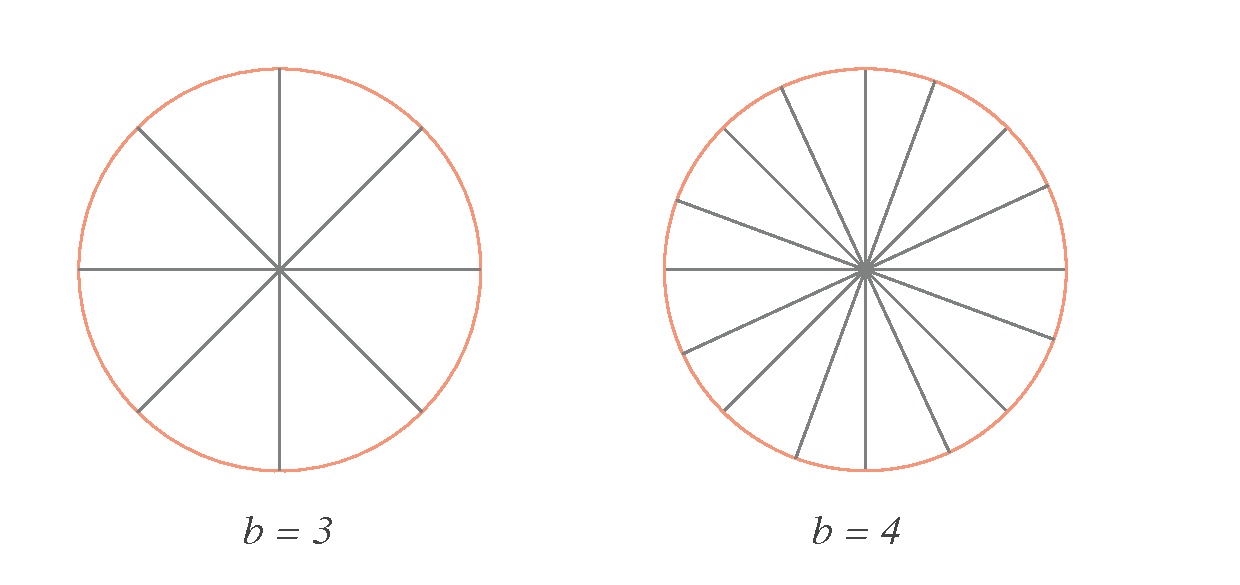
\includegraphics[width=0.9\textwidth, trim={0cm 0cm 0cm 0cm},clip]{illustrations/Lightlanes.jpg}}
%\subcaptionbox{$ 2r =\sqrt{2}L$  \label{xystion-simple-grid-ratio}}
\caption{Spherical emitter with Lightlanes at increasing values for $b$}
\label{fig:sphericalEmitter}
\end{figure}


\subsection{L - Lightlane coverage}
Lightlane coverage is a scalar taking the total area of the cross section of all lightlanes divided by the total area of the surface of a sphere at distance $D$. It can also be read as the expected number of lightlanes you will intersect at a randomly chosen position, at distance $D$. $r_e$ is the radius of the emitting sphere,  $\pi r_e^2$ its cross section, multiplied by $2^b$ lightlanes. At distance $D$, the lightlanes are intersecting a sphere with surface area $4\pi D^2$. The Lightlane Coverage is the ratio between these two areas. 

\begin{equation}
L(\nu) = \frac{2^{b(\nu)} \pi r_e^2}{4\pi D^2}
\label{eq:L}
\end{equation}

Notice that as $\lim_{d \rightarrow \infty}$, the denominator dominates. When $L = 1$, you will be receiving from an average of exactly one lightlane.  However, as you can see in Figure \ref{fig:darkZoneDistance}, even with regularized angle distance between lightlanes, small pockets between lightlanes have no coverage, other pockets lets you receive from two lightlanes. When $L=1$, the \textbf{low lightlane count} in this case 0 and the high lightlane count (in this case 2) occupy the same area of the sphere at distance $d$, and therefore they cancel out leaving $L =1$.

\begin{figure}
\centering
%\subcaptionbox{$ 2r =\sqrt{2}L$  \label{xystion-simple-grid-ratio}}
{\includegraphics[width=0.6\textwidth, trim={0cm 0cm 0cm 0cm},clip]{illustrations/LIghtlanesDZDistance}}
%\subcaptionbox{$ 2r =\sqrt{2}L$  \label{xystion-simple-grid-ratio}}
\caption{Dark zone distance - overlaid circles which exactly matches $L = \frac{2^b \pi r_e^2}{4\pi d^2} = 1$}
\label{fig:darkZoneDistance}
\end{figure}

\subsection{Tracking Coverage Area}
Suppose a telescope is orbiting the emitter. The Telescope has an onboard camera which has time-resolution  of $s$ seconds. A reference value could be $0.003$ seconds, which is the row-readout time of the XMM Newton onboard X-ray CCD, i.e $3$ milliseconds. However, because the telescope is moving, it might be passing in and out of Lightlanes. The area tracked by the Telescope during $s$ must be equal to it's speed times the diameter plus the area of the telescope lens. Let $r_d$ be telescope radius, $| \vec{v_e} - \vec{v_d} |$  be the relative velocity tangential to the emitter (in m/s).

\begin{equation}
TCA = \pi r_d^2 + s (| \vec{v_e}-\vec{v_d} |) 2r_d 
\label{eq:TCA}
\end{equation}



\subsection{Correction term}
The telescope may track a large area, but it's still only an effective diameter of $\pi r_d^2$. The correction term $\lambda = $ scales the area of the TCA back down to the real area of the telescope lens. 

\begin{equation}
\lambda =\frac{\pi r_d^2}{TCA} =
 \frac{\pi r_d^2}{\pi r_d^2 + s (| \vec{v_e}-\vec{v_d} |)  2r_d}	
\label{eq:lambda}
\end{equation}



\subsection{Lightlane density}

Let the number of photons that are travelling through each lightlane be given by the total number of emitted photons $E(\nu)$ per unit of time, divided evenly across the $2^{b(\nu)}$ available lightlanes. We assume a unknown relation so that $b$ is a function of $\nu$.

\begin{equation}
\gamma_L(\nu) = \frac{E(\nu)}{\pi r_e^2 2^{b(\nu)}}
\label{eq:gamma_L}
\end{equation}

Notice that instead of directly obtaining the photon density at sphere shell size ($4\pi D^2$), we divide the emitted photons by the sum of the Lightlane  cross sections.  ($2^b4\pi r_e^2$). In the limit of $\lim_{b \rightarrow \infty}$ these will become equilvalent, as we will proceed to show.

\subsection{Expected photon count equation}
We already found the Expected Photon count in the continuum limit being equal to $\hat{\gamma}_C(\nu)$, in equation :\ref{eq:gammaC}. The Lightlane counterpart is composed of the terms just introduced. 

\begin{equation}
\hat{\gamma}_L(\nu) = s \left( \gamma_L(\nu) \cdot L \cdot  TCA \cdot \lambda \right) 
\label{eq:expectedPhotonsFull}
\end{equation}
This can be read as the density of photons in each lightlane at $\gamma_L(\nu)$, multiplied by the expected number of Lightlanes we will intersect with at distance $D$. This is then multiplied by the telescope coverage area as it moves through space for the duration $s$. The final term $\lambda$ deflates the expected value to match the actual size of the telescope lens relative to the TCA.

Putting these together we get:
\begin{equation}
\hat{\gamma}_L(\nu) =   s\left( \frac{E(\nu)}{\pi r_e^2 2^{b(\nu)}}
	\cdot   \frac{2^{b(\nu)} \pi r_e^2 } {4 \pi D^2} 
    \left(  \pi r_d^2+ s (| \vec{v_e}-\vec{v_d} |)  2r_d \right)
	\cdot \frac{\pi r_d^2}{\pi r_d^2 + s (| \vec{v_e}-\vec{v_d} |)   2r_d }	\right)
\end{equation}

\subsection{Lightlane equality}
For the Lightlane quantization to be valid, it must match the continous derivation in the continous limit. 

\begin{equation}
 \hat{\gamma}_C(\nu)  = \hat{\gamma}_L(\nu) \\
 \label{eq:LightlaneEquality}
\end{equation}

Expanding the $\hat{\gamma}_C$ and $\hat{\gamma}_L$ into:

\begin{equation}
 s\left( E(\nu) \frac{\pi r_d^2}{4\pi D^2}\right)  = 
 s\left( 
 	\frac{E(\nu)}{\pi r_e^2 2^{b(\nu)}}  
 	\cdot   \frac{2^{b(\nu)} \pi r_e^2 } {4 \pi D^2} 
 	\cdot \left(  \pi r_d^2+ s (| \vec{v_e}-\vec{v_d} |)  2r_d \right)
	\cdot \frac{\pi r_d^2}{\pi r_d^2 + s (| \vec{v_e}-\vec{v_d} |)   2r_d }	\right) \\
\end{equation}

Due to cancellations:

\begin{equation}
\hat{\gamma}_C(\nu)  = \hat{\gamma}_L(\nu) = s\left( E(\nu) \frac{\pi r_d^2}{4\pi D^2}\right)
\label{eq:gammaL} 
\end{equation}

Comparing the simplified form of \eqref{eq:gammaL} to \eqref{eq:gammaC}, they are identical. The $\hat{\gamma}_L$ is the mean density, equal to $\hat{\gamma}_C$. 

There is nothing magical here, we just quantize and reverse the quantization. Notice that increasing Lightlane resolution ( $b(\nu)$, longer shutter time $s$ or faster comoving speed $|\vec{v_e} - \vec{v_d}|$, and reduced distance $r_d$ all contribute to reducing the difference between the continuum and the Lightlane formulations.  However, just like in the Lightlane Conjecture (\citep{RhadamantysA2}), the equivalence of the mean doesn't doesn't hold for the variance. 

\subsection{Variance in 3D}
In the previous paper , the variance equation for 2D was derived, see Eq : \ref{eq:TwinkleVariance2} in The Lightlane Conjecture.\cite{RhadamantysA2}.

\begin{equation}
	\sigma_L^2 = \left(E\left(p_r \cdot (\frac{L+1}{2^b}) + (1-p_r) \cdot (\frac{L}{2^b}) \right)- \gamma_C \right)^2
	\label{eq:TwinkleVariance2}
\end{equation}

This can be understood as constraints on how much a deviation from the continuum expected photon count $\hat{\gamma_C}(\nu)$ that can be explained by directional constraints on light. The Lightlane variance $\sigma_L^2$  is a contribution to the overall variance, separate from the variance caused other factors such as poissonian noise.

In 3D this is more complex. There will be one term of contribution to the variance for each integer value of $L$. As shown in \ref{fig:densityIsotropy}, the angle of the telescope relative to the grid affects the variability and the periodic pattern. As long as the detector is moving in a linear line relative to the projected grid, the result must be a periodic signal, such as that visualized in \ref{fig:observedFluxL3}. However, as shown in Fig \ref{fig:observedFluxHigh}, the Poissonian noise quickly dominates as the $\frac{L}{L+1}$ approaches unity. 

Because the variance depend has more terms, depends on the angle $\theta$ is \ref{fig:densityIsotropy}, it is well beyond my  abilities to formulate an analytic expression for the variance in 3D. However, in 2D, the variance contribution could be constrained between an upper and a lower bound. The bounds and their probability are subject to the number of lightlanes at point $n$, and $m$ is the remainder $m = n \mod 2$, corresponding to the most-dark-zoned and least dark-zoned trajectories of the camera.

Maximum dark-zoned area:
\begin{equation}
\underline{\sigma_L^2} 
 = \left(E\left((n / 2)  \cdot \frac{L+1}{2^b})
  + (n - n/2   +m) \cdot \frac{L}{2^b} \right) - \hat{\gamma_c} \right)^2
	\label{eq:TwinkleVariance3}
\end{equation}
Minimum dark-zoned are 
\begin{equation}
\overline{\sigma_L^2}
	 = \left(E\left(n-(n / 2) + m) \cdot \frac{L+1}{2^b} + (n/2   ) \cdot \frac{L}{2^b} \right)- \hat{\gamma_c} \right)^2
	\label{eq:TwinkleVariance4}
\end{equation}

\section{Computing the Lightlane grid size}
The remainder of this paper is devoted to studying the difference between $\hat{\gamma}_C$ and $\hat{\gamma}_L$ and their variance derivatives in situations where the $b$ is low enough to introduce noise. We will do this party using simulations in python.

In order to simulate a telescope receiving from lightlanes, we consider a large distance $r_d$ from an emitter, so that we can assume a locally flat patch of this sphere which the telescope moves across. This allows us to convert the 3D version back into 2D. Let the patch be of equal width and length, and area $|\vec{v}|^2 t$, where $|\vec{v}|$ is the velocity of the telescope (tangential to the emitter centre) and $t$ is the how long the observation lasts. Notice that $t > s$, so we will obtain a time-series of datapoints with $\frac{t}{s}$ points, each frame collecting photons for $s$ seconds. Our cylindrical lightlanes has become circular cross-sections placed side by side on the (locally) flat surface. The lightlanes can be closely spaced and overlapping (for high values of $b$), or far apart and not touching (for lower values of $b$). In order to place these circles we need to calculate the distance between the lightlane centers. It turns out the problem is same as the the ancient problem of squaring  the circle, where $(\sqrt{\pi})^2 = \pi r^2$, when $r = 1$. (Shoutout to Anaxagoras who built on previous Babylonian work while imprisoned).

Recall that $L$ was the expected number of lightlanes to intersect with for a randomly chosen point in the patch. Let $\underline{G_L}$ be the shortest distance between centers of evenly spaced lightlanes (a in \ref{fig:omegaRate}). Due to squaring of the circle when $L = 1$, the radius that ensures $L =1$ equals:

\begin{figure}
\centering
%\subcaptionbox{$ 2r =\sqrt{2}L$  \label{xystion-simple-grid-ratio}}
{\includegraphics[width=0.6\textwidth, trim={0cm 0cm 0cm 0cm},clip]{illustrations/OmegaRate.pdf}}
%\subcaptionbox{$ 2r =\sqrt{2}L$  \label{xystion-simple-grid-ratio}}
\caption{L = 1 when dark zone are (black) and Lucky Lanes area (yellow) have the same area}
\label{fig:omegaRate}
\end{figure}


\begin{equation}
\underline{G_L} =  2 \frac{\sqrt{\pi}}{2}r_e  = \sqrt{\pi}r_e
\label{eq:underline_G_L}
\end{equation}

The maximum distance $\overline{G_L}$ corresponds to taking the hypotenuse as in  $\sqrt{2}\underline{G_L}, $ Fig: \ref{fig:omegaRate}, right panel.
\begin{equation}
\overline{G_L} = \sqrt{2}\sqrt{\pi}r_e
\label{eq:overline_G_L}
\end{equation}

Because  $L$ (Lightlane Coverage) \eqref{eq:L} is the sphere shell express in lightlanes, i.e the expected number of lightlanes that overlap, the $\underline{G_L}$ is also a function of $L$:

\begin{equation}
\underline{G_L}(L, r_e) = \frac{\sqrt{\pi}r_e}{\sqrt{L}} 
\end{equation}
Inserting for $L$ yields

\begin{equation}
\underline{G_L}(r_e, b, d)
= 
\frac{\sqrt{\pi}r_e}{\frac{2^b \pi {r_e}^2 }{4\pi D^2}} 
=
\frac{2\pi D^2 \sqrt{\pi}r_e}{2^b \pi {r_e}^2 } 
= 
\frac{ d^2 \sqrt{\pi}}{2^{b+1}  r_e } 
\end{equation}

As a perchance useful tool, we can derive an expression for the distance $D$ associated with a given Lightlane Coverage. Let $L'$ be the desired coverage. 

\begin{equation}
\frac{2^b \pi {r_e}^2 }{4\pi D^2}  = L'
\end{equation}
Solving for $D$ yields:
\begin{equation}
D = \sqrt{\frac{2^{b-2}r_e^2}{L'}}
\label{eq:distance_to_star}
\end{equation}


\section{Lightlane photon density function }
As we are observing photon at the locally flat plane that hits the detector at distance $D$, we can remove the radial dimension and generate a 2D grid the camerea travel accros, see fig \ref{fig:gridOverlay2}. The distance between circles positioned at the distance $\underline{G_L}$, equation \eqref{eq:LightlaneEquality}, see in fig. \ref{fig:densityIsotropy}. The result is a density function of where the photons are equal probability inside each circle. Overlapping circles will have integer increases to the probability of detecting a photon. A detector passing through such a grid will have an angle $\theta$ relative to the orientation of this grid, with distinct patterns depending the angle it cuts through the lightlane density function. 

As shown in Figure \ref{fig:densityIsotropy}, the angle $\theta$ of the trajectory cutting through the circles affects the number of received photons. Provided sufficiently low $b$ or high $r_d$, this can affect the variability of the observed flux. The red arrow minimizes the time passing through dark-zone areas, which leads to a steady collection with small boosts at regular intervals. The blue arrow passes through dark zones between lanes, and has a lower total amount of photons received. Unlike the 2D version, the mean Luminousity will depend somewhat on this angle $\theta$, making the estimation of variance and mean quite complex.

It is also possible that a real telescope might transition from a "Lucky Lane" alignment with the grid at some point, into a "Dark Zone" alignment at other times, by having a curved trajectory. The telescope could be moving from overperforming into underperforming angles as a result of relative movement. This should repeat at larger time-series duration, buton shorter durations, this can only manifest as quasi-periodicity that is unstable and unpredictable because it depends on change in the unknown $\theta$  parameters. 

\begin{figure}
\centering
%\subcaptionbox{$ 2r =\sqrt{2}L$  \label{xystion-simple-grid-ratio}}
{\includegraphics[width=1\textwidth, trim={0cm 0cm 0cm 0cm},clip]{illustrations/LaneGrid.pdf}}
%\subcaptionbox{$ 2r =\sqrt{2}L$  \label{xystion-simple-grid-ratio}}
\caption{Anisotropic flux variability of telescope}
\label{fig:densityIsotropy}
\end{figure}

This also applies to another confounding factor that affect the lightlane cross-section radius. In this paper we assume that lightlanes are not \textbf{expanding}. This is clearly wrong. Light from distant galaxies are known to be redshifted and also passing through interstellar dust. Possibly the former but certainly the latter generate scattering. The result is that any lightlanes signal become conical as their radius increases linearly with the distance $D$. They are also obviously weakened by the same effect. This would weaken any signal significantly, contributing to the Lightlane Equality. There are several other factors to boot, see section confounding variables for a list of reason why the a Lightlane signal can be very difficult to detect.

\section{ Simulating flux variability : Results}
Not having the skills to create an analytic expression for the variance in 3D, I have  attempted to simulate a moving telescope camera across a the Lightlane density function. It is possible that despite all sources of noise, a statistical signal from Lightlanes might be observable. However, we must address the most important type of noise in the stochastic sampling - Poissonian noise. In current astrophysics, the Poissonnian noise assumed to be the only light-transport component to variance. Other sources of noise are thought to come from the variability of the brightness of the star itself, dust clouds etc.

\subsection{Poissoninan noise Monte-Carlo}
The Poissonian noise is simple reproduce using a Monte Carlo method. We are adding the Lightlane Variability on top. We simulate a puny star with diameter of $10$km, at a distance of $D =10240$ kilometers from the emitter centre. We ignore the radius of the planet. To compute the probability of a photon hitting the detector during the shutter time $s$ we use the letter $p$. It is equal to the size of the detector relative to the lightlane cross section, multiplied by expected number of lightlanes that it can receive from ($L$), this is multiplied by the density of photons in each Lightlane $\frac{E}{2^b(\nu)}$.

\begin{equation}
p = \frac{\pi r_d^2}{\pi r_e^2}L(\nu) \frac{ E(\nu)}{2^{b(\nu)}} s
\end{equation}
Where $\frac{\pi r_d^2}{\pi r_e^2}$ is the size of the detector compared to the Lightlane Cross section. $L(\nu) $ is the Lightlane coverage for this wavelength interval ,(\eqref{eq:L}) and $\frac{ E(\nu)}{2^{b(\nu)}}s$ is the density of photons in each lightlane volume. 

Monte Carlo method randomly samples according to this probability density, which means that the detected photons obey Poissonian statistics.
An approximation to the poisson distribution can be made by:
\begin{equation}
\gamma_t = s H \sum_{n = 1}^{max = \infty} p_{\lambda}^n
\end{equation}

For our simualtion, we have a probability of $p \approx 0.01$, we can set the $max = 5$ to get a $1e-6$ probability of missing something. The telescope trajectory passes through lightlanes is illustrated in \ref{fig:observedFluxL1} (a). The resulting flux is visualized in Fig. \ref{fig:observedFluxL1} (b)

\begin{figure}
\centering

 \begin{subfigure}[t]{0.45\textwidth}
       
{\includegraphics[width=1\textwidth, trim={0cm 0cm 0cm 0cm},clip]{../../Variance/py/img/L1B44A30_Circles.jpg}}

\caption{Telescope trajectory $L = 1$}
\label{fig:telescopeTrajectory}
 \end{subfigure}
 \begin{subfigure}[t]{0.5\textwidth}
{\includegraphics[width=1\textwidth, trim={0cm 0cm 0cm 0cm},clip]{../../Variance/py/img/L1B44A30_CountsL.jpg}}
%\subcaptionbox{$ 2r =\sqrt{2}L$  \label{xystion-simple-grid-ratio}}
\caption{Observed flux from telescope}
\label{fig:observedFlux}
\end{subfigure}
\caption{Flux variability for $L =1$, distance $D = $ 20 971 520 km}
\label{fig:observedFluxL1}
\end{figure}

\begin{figure}
\centering

 \begin{subfigure}[t]{0.45\textwidth}
       
{\includegraphics[width=1\textwidth, trim={0cm 0cm 0cm 0cm},clip]{../../Variance/py/img/L3B44A30_Circles.jpg}}

\caption{Telescope trajectory $L =3$}
\label{fig:telescopeTrajectoryL3A}
 \end{subfigure}
 \begin{subfigure}[t]{0.5\textwidth}
{\includegraphics[width=1\textwidth, trim={0cm 0cm 0cm 0cm},clip]{../../Variance/py/img/L3B44A30_CountsL.jpg}}
%\subcaptionbox{$ 2r =\sqrt{2}L$  \label{xystion-simple-grid-ratio}}
\caption{Observed flux from telescope}
\label{fig:observedFluxL3B}
\end{subfigure}
\caption{Observed flux $L=3$, distance $D$ = 12 107 912 km}
\label{fig:observedFluxL3}
\end{figure}



\begin{figure}
\centering

 \begin{subfigure}[t]{0.45\textwidth}
       
{\includegraphics[width=1\textwidth, trim={0cm 0cm 0cm 0cm},clip]{../../Variance/py/img/L672B48A30D3235975_CountsL.jpg}}

\caption{b = 48, D = 3 235 975 km }
\label{fig:telescopeTrajectory}
 \end{subfigure}
 \begin{subfigure}[t]{0.5\textwidth}
{\includegraphics[width=1\textwidth, trim={0cm 0cm 0cm 0cm},clip]{../../Variance/py/img/L21B43A30D3235975_CountsL.jpg}}
%\subcaptionbox{$ 2r =\sqrt{2}L$  \label{xystion-simple-grid-ratio}}
\caption{b = 43, D = w3 235 975 km }
\label{fig:observedFlux}
\end{subfigure}
\caption{High bitlength, distance $D$ = 3 235 975 km}
\label{fig:observedFluxHigh}
\end{figure}

In Figure \ref{fig:observedFluxL3}, increasing the desired LaneCount to $L = 3$ we see more noise. In Fig \ref{fig:observedFluxHigh} we hold the distance constant, and only adjust amount information available for direction to $b = 48$. By reducing $b$ significantly to 43, we see much stronger flux variability. We can see that the stochastic sampling process hides the correlation between the lightlane and the flux. 

\section{Conclusion}

The constraint on directional freedom for photons, means that the Lightlane equations predicts an additional component to flux variability, originating from the constrains on directional freedom. However, this component could be very small, and it is likely that if it was large, it would easily have shown up in fourier transforms previously. Lightlane equations also suggest that if the degree of overlap between lightlanes $L$ is high, like in Fig. \ref{fig:observedFluxHigh}, the length of the exposure window $s$, might be long enough to obscure the effects completely even when $s < 3ms$, owing to the lightlane equality $\hat{\gamma_C} = \hat{\gamma_L}$. Furthermore, there is reason to believe that the variability component should increase into the high-energy spectrum, provided an inverse relationship between bitlength $b$ and frequency. There is reason to assume such a inverse relation, but the reasoning  underpinning this suspicion goes deep into the the information exchange mechanism of the Serpentine class CA, and is not in scope for this paper.

In combination, Lightlane theory predicts a small but increasing flux-variability component as wavelength is reduced. However, there are many effects that would weaken this signal, if it exists. An obvious one would be interstellar dust and atmospheric scattering. Averaging different wavelengths using a smoothing filter might combine wavelenghts with different Lightlane projections, effectively increasing the resolution of the projection, and therefore reducing the possibility of detecting as signal. Finally, magnetic and sun-spot related activity which are the major constituents of stellar flux have strong variability, and can easily explain the magnitude of the scattering itself. Finally, separating Lightlane Flux Variability from noise gets increasingly difficult experimentally, particularly if we find that we need to use small frequency bands $d\nu$. 


\subsection{Confounding factors}
As mentioned, a straight path across an evenly spaced lightlane sheet will result in quasi-periodicity in the variance. While this must be periodic on larger time scales, finding this might be difficult to detect, as it would be correlated in a very complex way with the trajectory of the telescope and the earth, as it's speed and position realizes different angles relative to the Lightlane Density function. In order to simulate such effects, the entire arena must be done in 3D including the orbital paths of the observer,  the comoving velocity of the target and any effects en route. In addition to being at best quasi-periodic, such systematic periodicity can be lost simply by the common practise of aggregating counts, stiching together of time-series taken at different times, folding or a myriad of reasons relating to the sensitivity of telescopes, shutter time $s$, moving shutter effects, post-processing, time averaging, rejected counts etc. 

The periodicity gets even more difficult to make sense of, if the camera is moving in a curved line across the Lightlane projection surface. This is very likely, because the orbit of telescopes are elliptical, and the orbit of the earth around the sun almost circular. 
Also, scattering from interstellar dust will contribute to enlarging the radius of the lightlanes, thus increasing L - and will also shift the wavelengths into lower energies, which have more lightlanes. Even so, redshift might be caused by the substrate of the universe growing, or the photon TCAs aquiring additional information ¨from this expansion mechanism as they propagate through space, or both. The latter possibility imply that light will be scattered by the cosmological expansion as well. All these arguments make it difficult to search for confirmation and falsification without adding very many new variables. As is typical for astronomy, the picture gets muddled very quickly. 
Because of all these effects contributing random factors, detecting periodicity in the variance might be limited certain subset of the available frequencies (i.e X-rays), or require emitters to be sufficiently far away, studying sufficiently luminous sources with enough luminousity in a narrow band to provide enough counts. 

However, these arguments also contribute to an explanation for why  periodicity in flux variability could have evaded detection so far. Without a model complex enough to cover unexplained quasi-periodicity, it will simply be classified as unexplainend flux variability,  blurring and sometimes quasi-periodic patterns depending on the timescale of the variability.  

Most studies of starlight spectra use Power Density Spectrums which are corrected and prepared from the Observation Data files, and few researchers work directly with high time-resolution time-series because they do not add any value and frequently have blank frames with noise only. 



\subsection{Conclusion}
Lightlane theory is an attempt to use an information theoretic approach to make contact between interpretations of Quantum Mechanics that rely on Cellular Automata, with telescope data. We show that under these constraints, a new source of flux variability must be present, however small. The approach required introducing several new variables and relations, notably $b(\nu)$. These variables are derived from information theoretic constraints which apply to all Digital Physics theories that place constraints on the directional freedom of movement for elementary particles. This means that the Cellular Automata Intepretation of Quantum Mechanics, presented by Gerard t'Hooft in 2014 \citep{hooft2014cellular} cannot be viable unless some amount  glitchyness is present in the flux data. Such variability must exist because completely continuous behaviour is an impossible task for a discrete TCA to perform. It's a big suprise to me that these constraints end end up  predicting complex quasiperiodic behaviour to the starlight flux variability. And because this quasiperiodicity is an artifact of the model, if such periodicity is found, then the theory stands to be taken seriously.

Lightlane theory also predicts many other effects that I have not had time to grapple with. One of them is blurring. Images of distance galaxies are likely to be blurred inn a way similar to how scaling of a low resolution image results in a blurry picture. This blurring effect comes in addition to that caused by interstellar dust. We know from \citep{2021dustdraine} that there exist an upper bound on how much of currently observed scattering that can be explained by interstellar dust, and that dust does not fully explain the extinction and blurriness observed. This will hopefully be adressed in a later paper.




\bibliographystyle{plain}
\bibliography{../mybib}
\end{document}

\subsection{Increasing flux variability with higher frequency}
Our model of the photon suggest that the variability is inversely related to the amount of information included in the Serpentine propagation program, low information photons will express more flux variability. Testing Lightlane theory using Flux Variability datasets would require us to estimate the error between the Expected (Poissonnian) and actual flux variability, using models which simulate the activity of the sun.

Suppose that shorter wavelength mean less information. In this case, we should see increased variability in the high-frequency spectrum. This is actually the case. Based on data from XMM Newton telescope Figure \ref{fig:epatplot}, data from the star $\Theta$ Aur has been fitted with data from an Strömgren photometric system, and corresponds to the best fit. Notice the tight fit in the low-energy spectrum, and the more jagged lines in in the high-energy ranges. This is related to a phenomenon distinct to X-ray telecsopes called pile-up, which possibly can allow for a statistical detection. It is possible that an overabundance of pile-up could be resulting from photons clustering into the same lightlane. This approach  avoids the problem of parametrizing complex periodicities, and let us study  (under some constraints) time resolutions even lower than the row-readout time $s$ of the onboard X-ray cameras of the XMM Newton and Chandra telescopes. So far I have only been able to ascertain, that there is far more pile-up than anyone can understand.


\begin{figure}
\centering
{\includegraphics[width=0.7\textwidth, trim={0cm 0cm 0cm 0cm},clip]{charts/epatplot_pileup.png}}
\caption{ Pile-up increasing with energy level }\label{fig:epatplot}
\vspace*{0.5in}
\end{figure}

This however, does not contradict Lightlane theory, only constrain it. Lightlane theory predicts a component to flux variability which is stronger in high-energy band.

This  have however, identified a phenomenon distinct to X-ray telecsopes called pile-up, which possibly can allow for a statistical detection. It is possible that an overabundance of pile-up could be resulting from photons clustering into the same lightlane. This approach  avoids the problem of parametrizing complex periodicities, and let us study  (under some constraints) time resolutions even lower than the row-readout time $s$ of the onboard X-ray cameras of the XMM Newton and Chandra telescopes. So far I have only been able to ascertain, that there is far more pile-up than anyone can understand.

\section{Prediction 1: Coruscating light from moving lightlanes}

\begin{figure}
\centering
{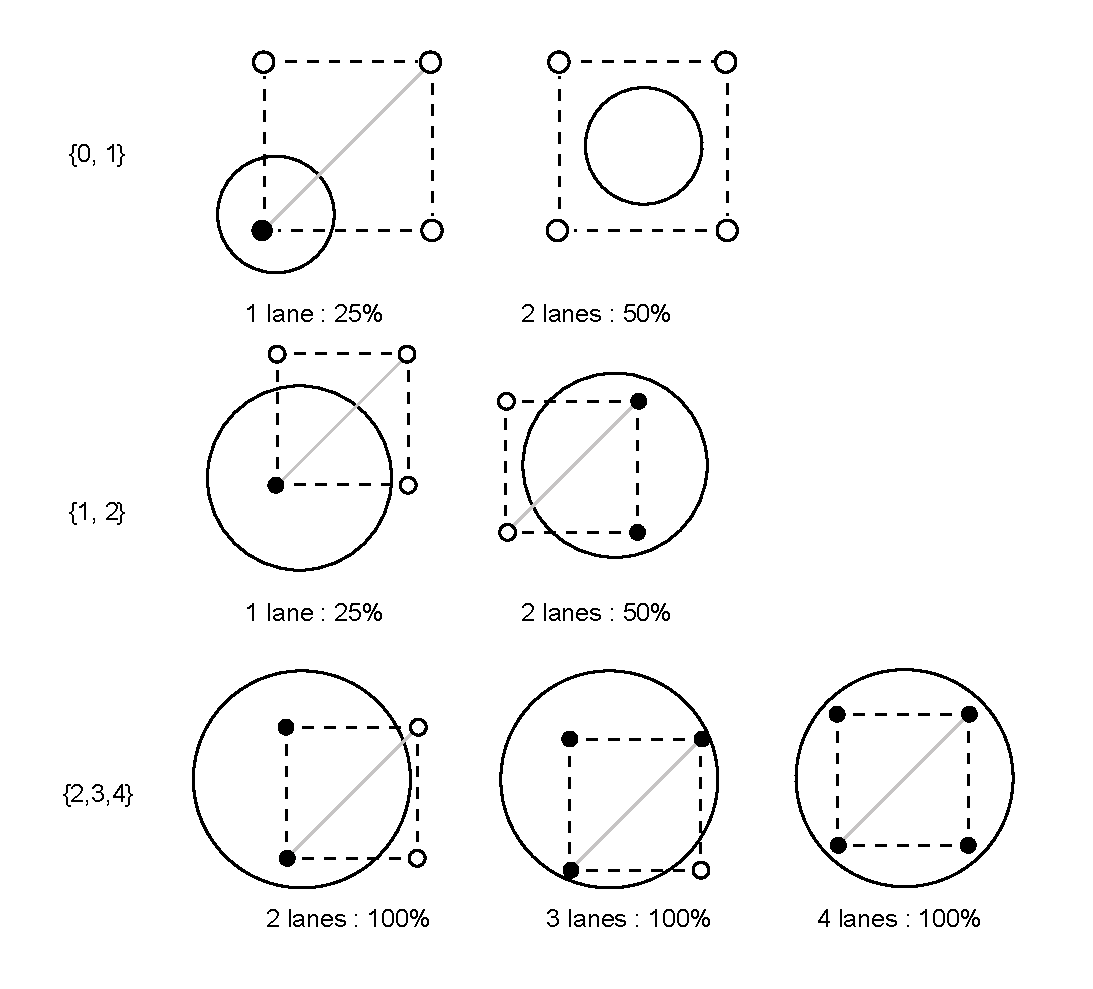
\includegraphics[width=0.7\textwidth, trim={0cm 12cm 0cm 0cm},clip]{illustrations/SimpleGridRatio1.pdf}}
\caption{ 0-1 "Occulting" cycle between $ 2r < \sqrt{G}  $. Alternates between 0 and 1 lightlane.   }\label{fig:OccultingTwinkler}
\vspace*{0.5in}
{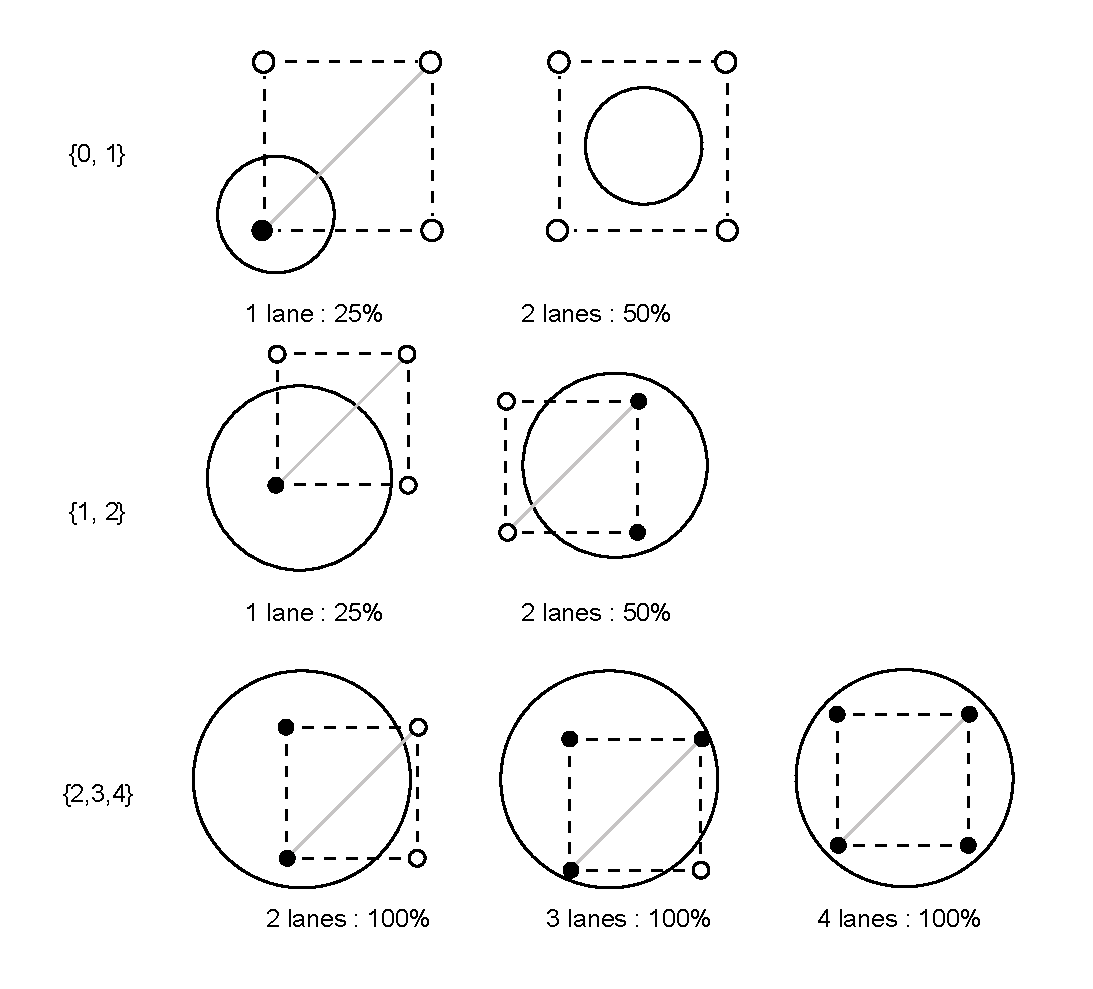
\includegraphics[width=0.7\textwidth, trim={0cm 6cm 0cm 5cm},clip]{illustrations/SimpleGridRatio1.pdf}}
\caption{ 1-2 cycle "half" cycle between $  \sqrt{G} < 2r < sqrt{2}\sqrt(G) $. Alternates between 1 and 2 lightlanes.}\label{fig:12cycle}
\vspace*{0.5in}
{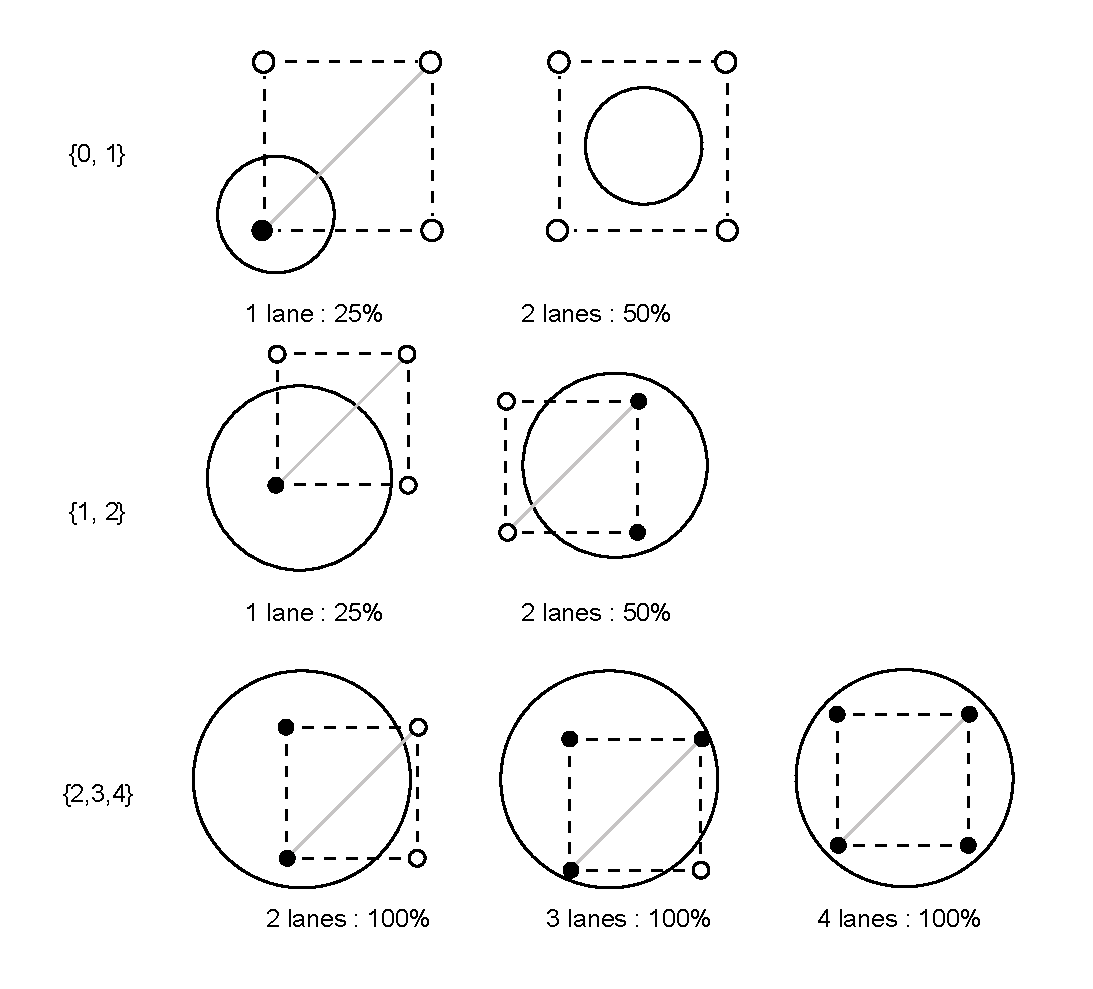
\includegraphics[width=0.7\textwidth, trim={0cm 0cm 0cm 10cm},clip]{illustrations/SimpleGridRatio1.pdf}}
\caption{ 2-3 cycle between $  \sqrt{2}\sqrt(G) < 2r < ... $. Alternates between 2, 3 (briefly) and 4 lightlanes.}\label{fig:12cycle}


\end{figure}

Coruscating is an old word meaning "to give forth intermittent or vibratory flashes of light; to shine with a quivering light". This is a beautiful wording of the first physical prediction of Lightlane theory, realized through the special class of probability density called "Twinkles" which was introduced in "Lightlane Equality" \citep{RhadamantysA2}.

We recall from the same paper how the equation for the Variance included the bitlength expression $2^b$, repeated here: \eqref{eq:deviancefrommean}.

\begin{equation}
\underline{\sigma^2} 
 = \left(E\left((n / 2)  \cdot \frac{((L+1)-\hat{L}}{2^b})
  + (n - n/2   +m) \cdot \frac{( L- \hat{L} )}{2^b} \right) - \hat{\tau_c} \right)^2
	\label{eq:TwinkleVariance2}
\end{equation}
\begin{equation}
\overline{\sigma^2}
	 = \left(E\left(n-(n / 2) + m) \cdot \frac{((L+1)-\hat{L})}{2^b} + (n/2   ) \cdot \frac{( L- \hat{L} )}{2^b} \right)- \hat{\tau_c} \right)^2
	\label{eq:TwinkleVariance2}
\end{equation}



The $K_i$  correspond to the number of simultaneous lightlanes intersecting the detector, and $P_i$ the probability of this occurence. In the previous paper, a very simple form of Twinkle was introduced, always coruscating between a high and low lightlane count, which are always adjacent integers. For example, if the expected lightlane $\hat{L} $ was given as 2.53, this would translate into receiving 3 lightlanes 53\% of the time, and two lightlanes 47\% of the time. In 2D, Twinkles are always two adjacent integers, not more not less.

It is important to note that in three dimensions, Twinkle densities  become more complex, and may even vary depending on the orientation of the detector and it's cross section. To understand how the calculation of the Expected number of lightlanes $\hat{L}$ and the resulting Twinkle affect radiance we start with the simplest case, using a circular detector oriented perfectly toward the source. 

In Figure \ref{fig:OccultingTwinkler} we have the most extreme case for circular detectors, the "Occulting" Twinkle. This occurs when the diameter of the detector (circle) is capturing light transported by the corners of each Grid cell (square) is less than the (overlaid) grid length $\sqrt{G} $. As we can see in figure \ref{fig:OccultingTwinkler} it may or may not intersect depending on position, intersecting with either 0 or 1 lightlane. This Twinkle pattern is similar to the simple Twinkle discussed in \citep{RhadamantysA2}. In the next Figure \ref{fig:12cycle}, we can see that when  $ \sqrt{G} =2 \sqrt{2}r$ all corners of the square touches the circle when the circle is perfectly centered inside the square. At this size intersecting with 4 corners is only possible as an edge case, and has 0\% probability. If we move the grid or detector around, it will intersect with two or one corners. 
Eventually as we reach the lowest threshold value of all$ 0 <  2r < L $ ,  we enter into the "Occulting" cycle {0,1} shown in figure \ref{fig:OccultingTwinkler}.

 


This demonstrates that there are distinct transition values between Twinkles, where values for the grid and the size of the detector transition from cycling between 1 and 2 lightlanes, and begin cycling between  0 and 1 lightlanes. Between these transition values the amount of light is modulated by the probabilites associated with each lightlane count. When such a probability reaches 0, it triggers a Twinkle shift point and another lanecount starts to rise from 0. Such transition points exist for each integer. The measured flux is smoothed between transition points by the amount of time that the detector spends intersecting the high number of lightlanes versus the low number of lightlanes in its current Twinkle. I.e : Let the detector have a size so that it intersects 2 lanes $ 30\% $ of the time, and 1 lane $ 70 \% $ of the time. The detector will be in the $ {1,2} $ the flux will be $0.3 E_L + 0.7 E_L $, where $ E_L  $ s the number of photons per lane, per unit of time.



\section{Prediction 2: Aggregate Dark zone}
Notice that the radius of the luminous object, the star or galaxy or whatever it is we are observing is not used in Equation \eqref{eq:Grid}. The reason for this is that we are estimating $\hat{L}$, the expected number of lightlanes intersecting the relevant part of the lens at a given time. The size of the object is indirectly specified through $\frac{\kappa}{\phi}$ and $d$, allowing us to calculate $G$.




But this does not mean that this overlaid grid $G$ is equally available everywhere. We remember from \citep{RhadamantysA2}, the concept of Dark Zone for point emitters in both two and three dimensions. (See Figure \ref{fig:pointEmitter2}). 

Eventually, at large enough distances we will see a solid equivalent of the "Dark Zone" and "Lucky lane". This occurs because the lightlanes extending from a solid eventually become so dispersed that they now travel in packs of perfectly parallel rays, carrying the same Directional Information but retaining their original offset from the time of emission. 

At such large distances, the radius of the luminous object enters the equation as a free parameter alongside bitlength $b$ and distance $d$. In practice this makes the lightlanes themselves coalesce into tubes with the exact same directional configuration, interspersed with areas of no light between them. The concept of DarkZone and "Lucky Lane" thus reappears at a different scale. In Figure  \ref{fig:hubbleDarkZone}, we can visualize our hubble telescope moving through such solid "tubes". 

This however, leads to some very strange predictions. For example, it is possible that a camera is capturing an image of a part of the sky, receiving light from a distant star. A year later, the same location in space is viewed, but the  star is completely gone without a trace! The result is that the telescope, hitching a ride on the earth has moved more than the diameter of the distant star,  left the current "lightpipe". For this to occur, the distance to the star must be such that the diameter of the "lightpipe" is approximately the same as the diameter of the dark-zone, so that there is a 50\% chance of detection vs / non-detection.



\section{ADASD}
Equation for the probability of a dark-zone.

The probability of a detector of a given size with a lightlane, is equal to the cross section of the emitter, divided by the hemisphere it faces. If this is bigger, then the classial interpretation holds.


\begin{equation}
	P_L = \frac{2^b \pi r^2 }{2 \pi D^2 } = \frac{2^b r^2}{ 2 D^2} 	
\label{eq:shareofhemispherewithinlightlane}
\end{equation}

The equation computes the total area covered by all lightlanes emitted from a spherical object (with a circular cross-section), when projected on the hemisphere at distance D. If this is actually larger than 1, any point within the surface an be reached of this current bitlength, so there is no dark zones. The integer part of $P_L$ represents the number of lightlanes it will intersect, and the decimal part equals the probability of intersecting with another one.

However, when the number is $0 < P_L < 1$, the number represents the share of the hemisphere covered by a lightlane. Assuming that the detector is tiny compared to the emitter, $P_L$ simply states the probability that the detector can see this frequency from this emitter at a given position in space. As we are dealing with moving emitters and detectors, this number translates into the fraction of the time that we are receiving light, versus the fraction of time we are in a dark-zone. 



\begin{figure}
\centering

\end{figure}



\begin{figure}
%\subcaptionbox{$ 2r =\sqrt{2}L$  \label{xystion-simple-grid-ratio}}
{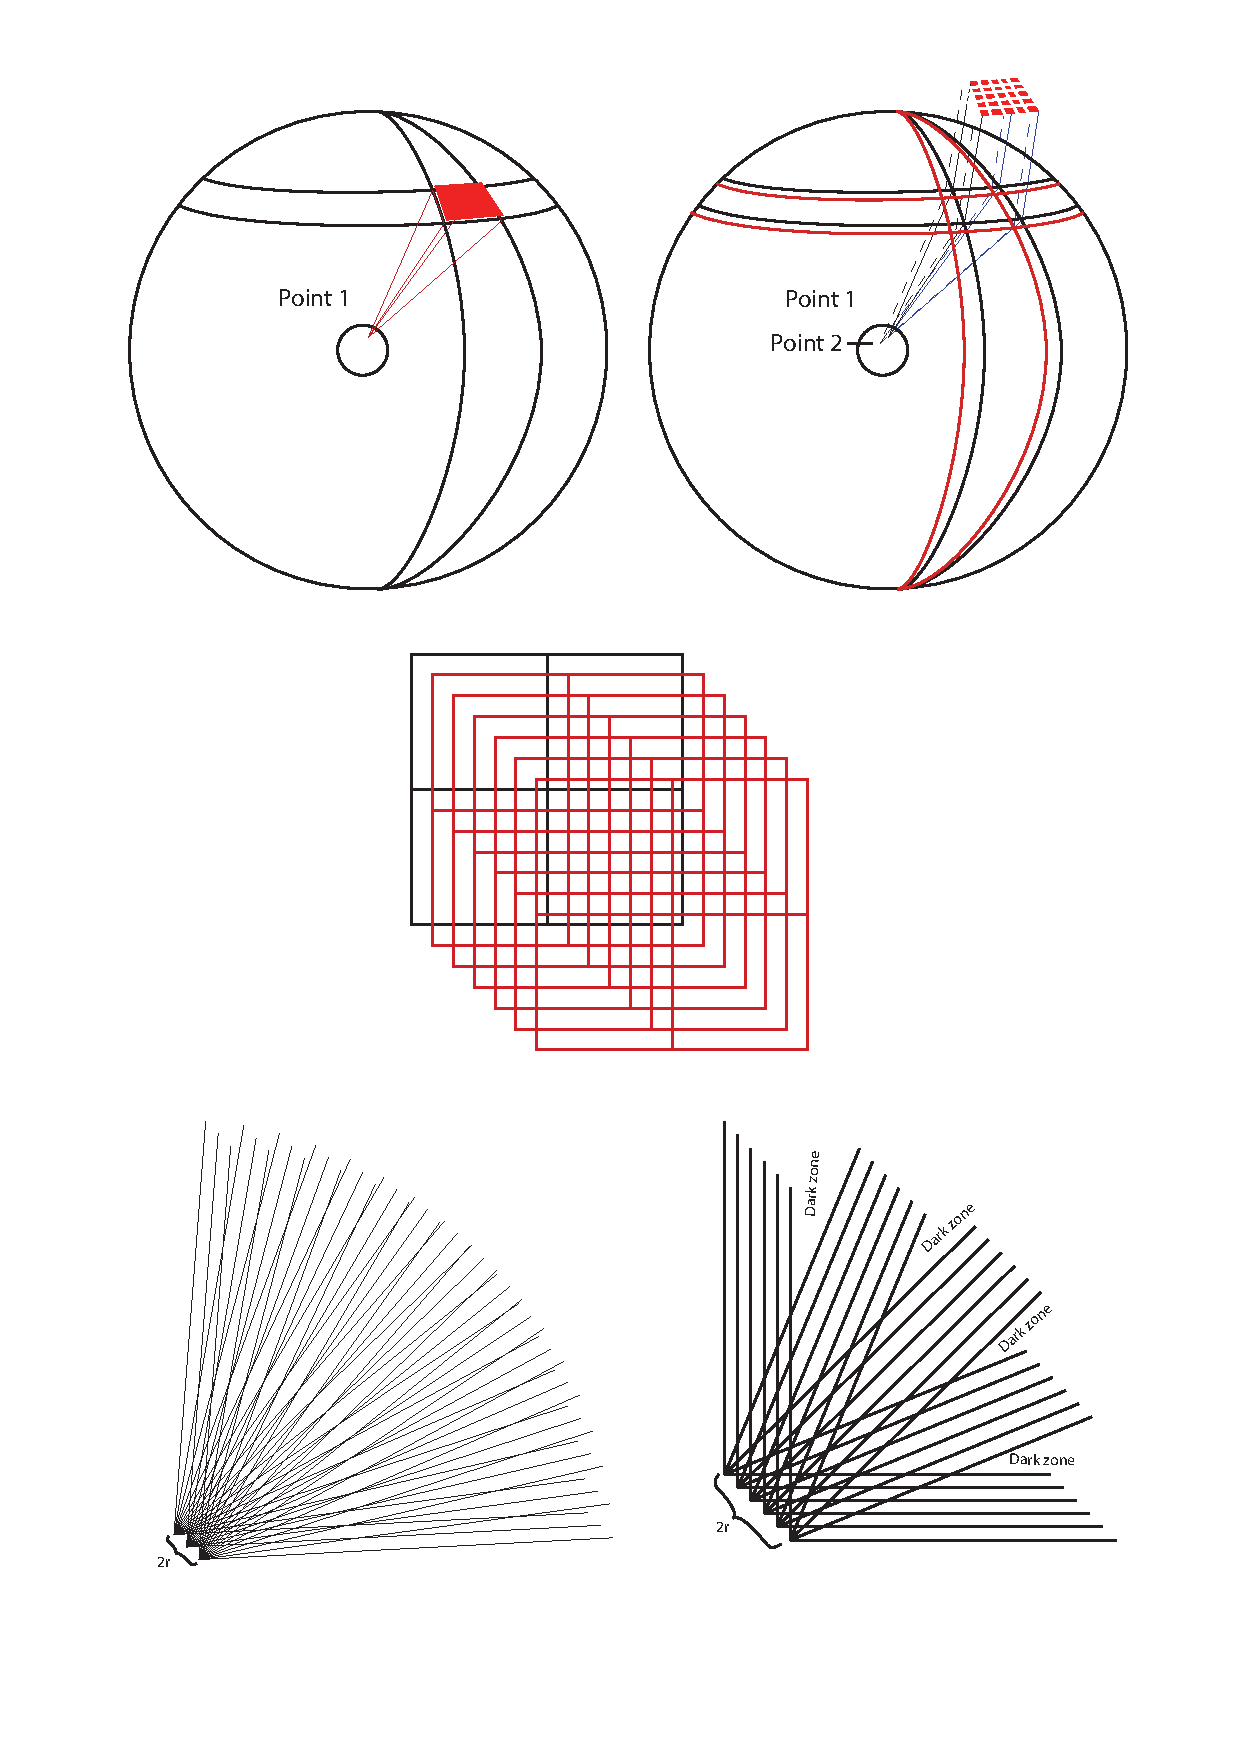
\includegraphics[width=0.8\textwidth, trim={0cm 19cm 0cm 0cm},clip]{illustrations/PointEmitterToBodyEmitter.pdf}}
%\subcaptionbox{$ 2r =\sqrt{2}L$  \label{xystion-simple-grid-ratio}}
\caption{The grid resulting from a low resolution point emitter. Additional point-emitters subdivide the grid, producing a finer grid }
\label{fig:gridOverlay1}
{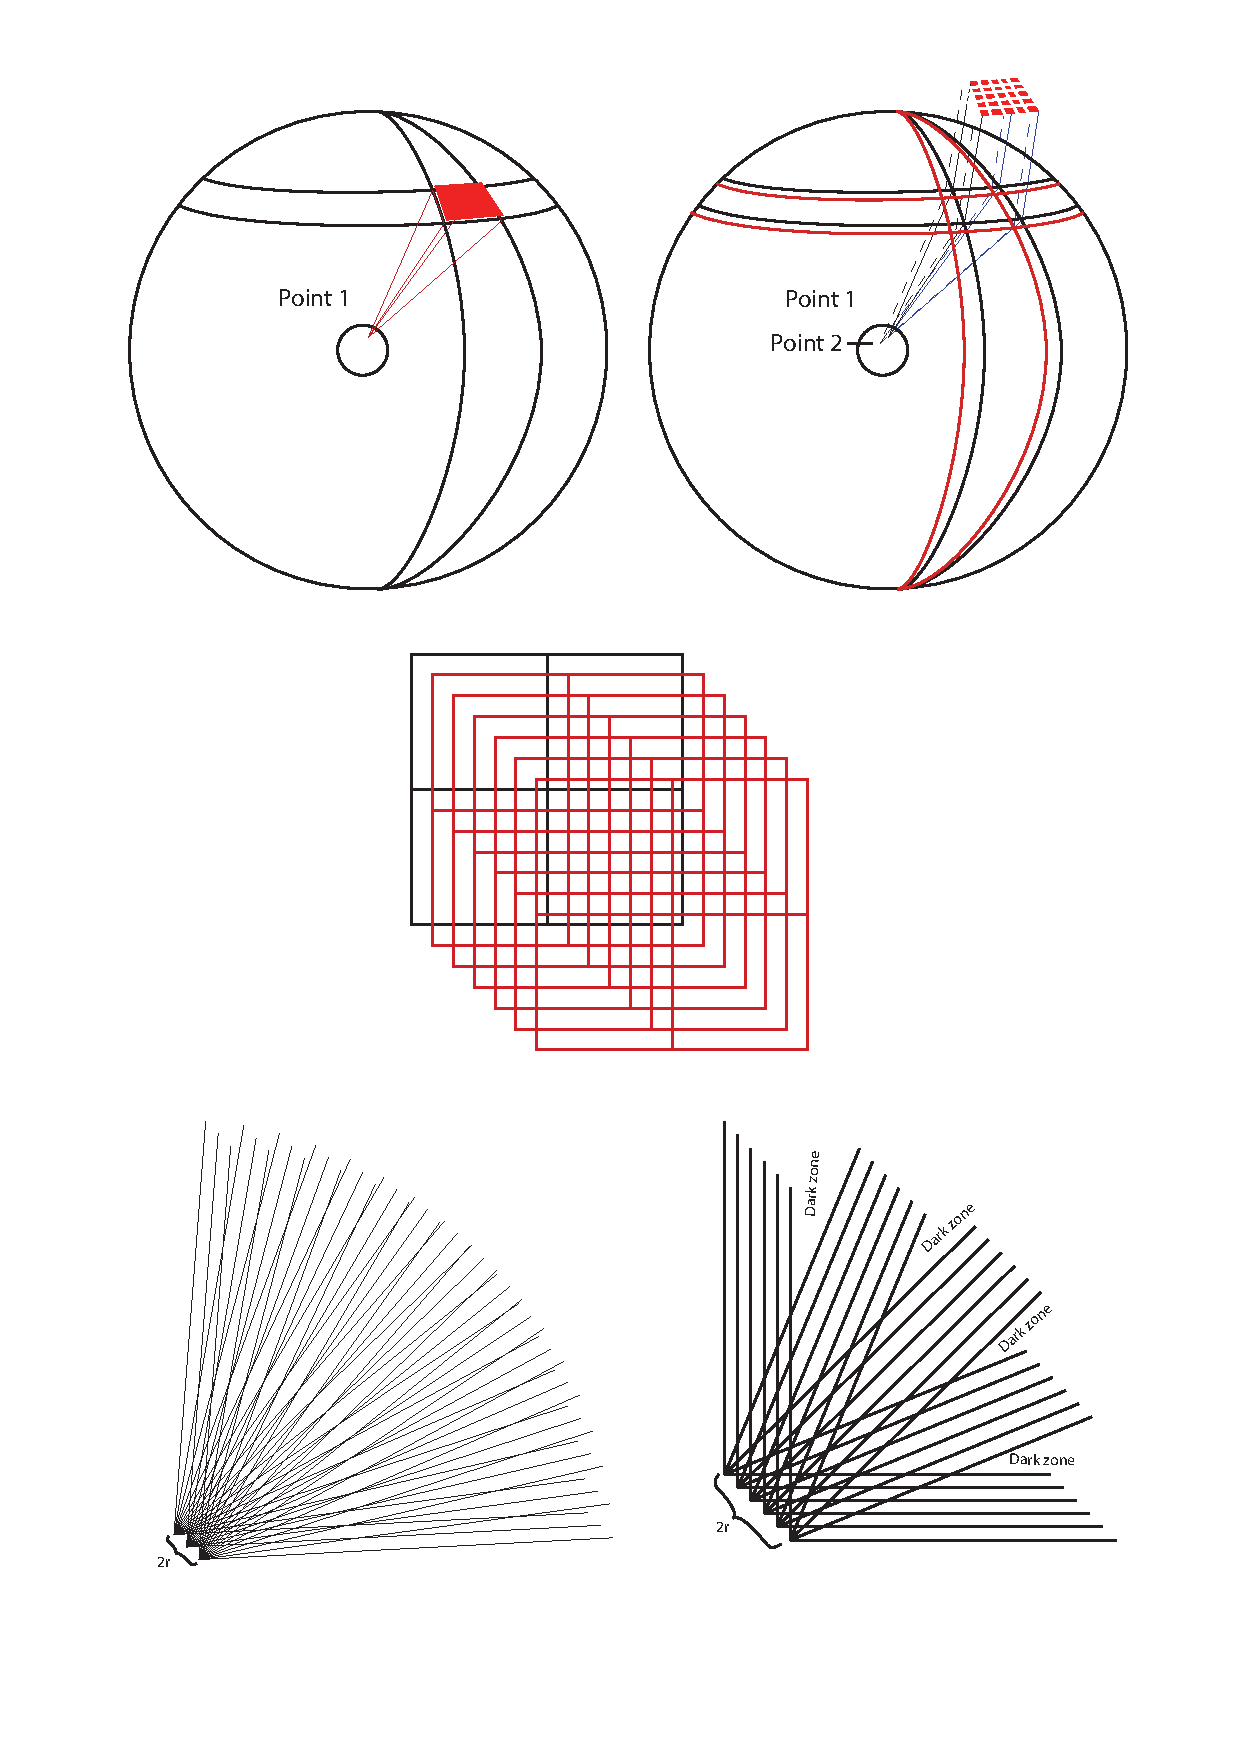
\includegraphics[width=0.8\textwidth, trim={0cm 11cm 0cm 10cm},clip]{illustrations/PointEmitterToBodyEmitter.pdf}}
%\subcaptionbox{$ 2r =\sqrt{2}L$  \label{xystion-simple-grid-ratio}}
\caption{Overlaid grid: Subdivided grid projection is the result of adjacent point emitters, each projecting a grid of bitlength $b$.  }\label{fig:gridOverlay2}
{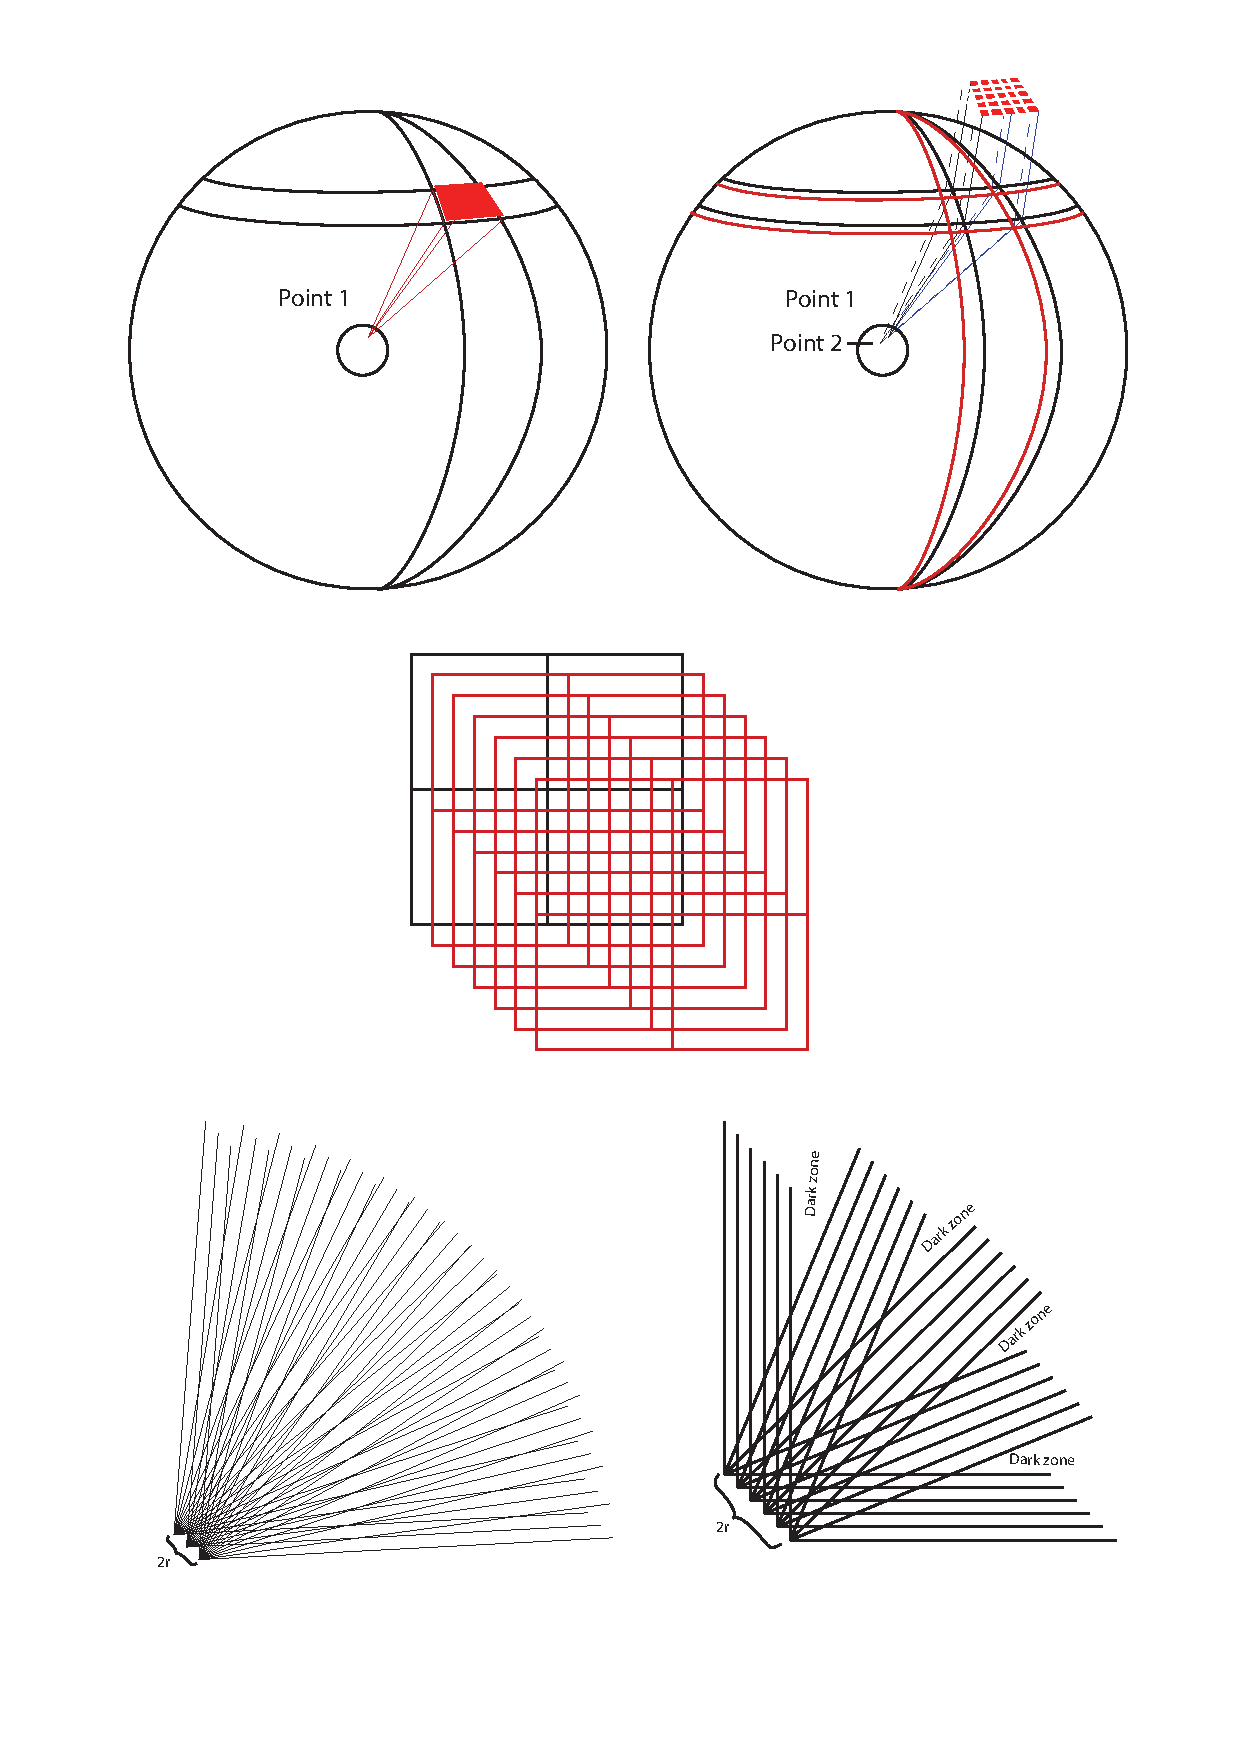
\includegraphics[width=0.8\textwidth, trim={0cm 2cm 0cm 18cm},clip]{illustrations/PointEmitterToBodyEmitter.pdf}}
%\subcaptionbox{$ 2r =\sqrt{2}L$  \label{xystion-simple-grid-ratio}}
\caption{Body emitters are point emitters which overlap until they reach the dark-zone wedge}\label{fig:solidDarkZone}

\end{figure}
%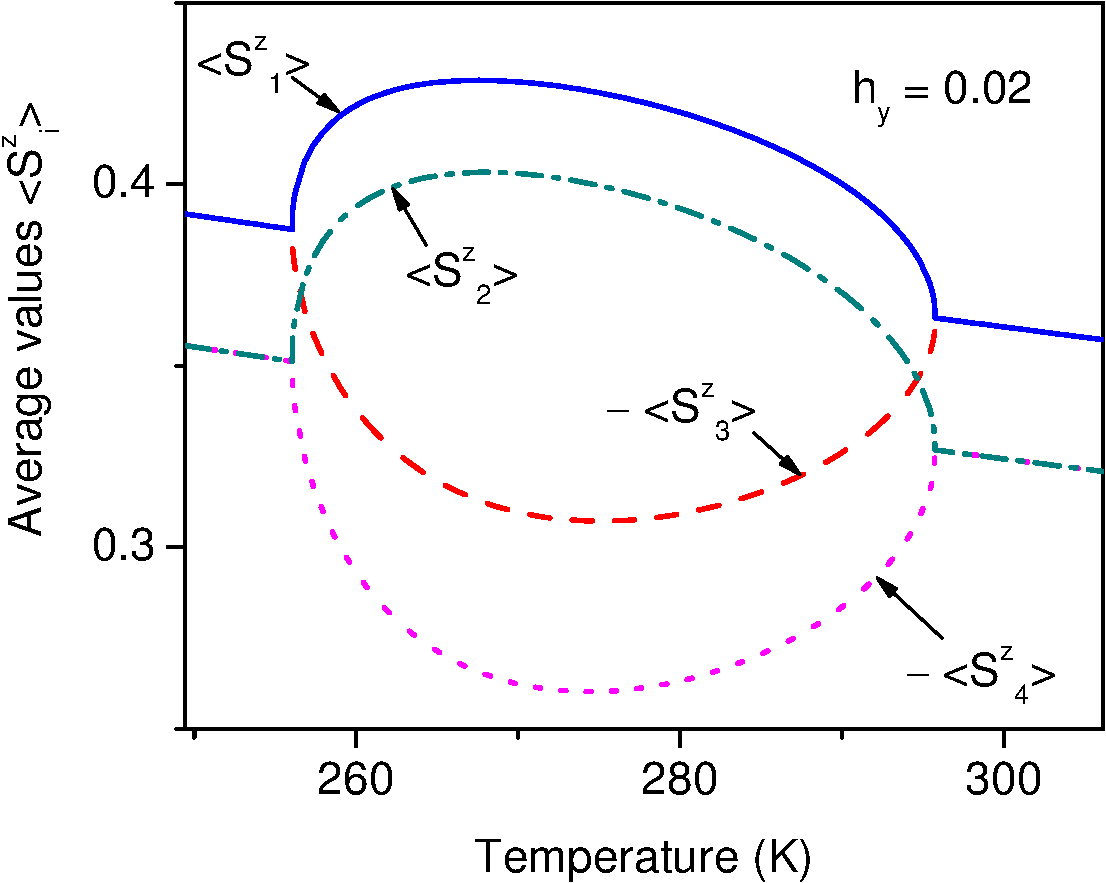
\includegraphics[width=0.65\textwidth]{eps_demo}
\begin{figure}
\centering
%\subcaptionbox{$ 2r =\sqrt{2}L$  \label{xystion-simple-grid-ratio}}
{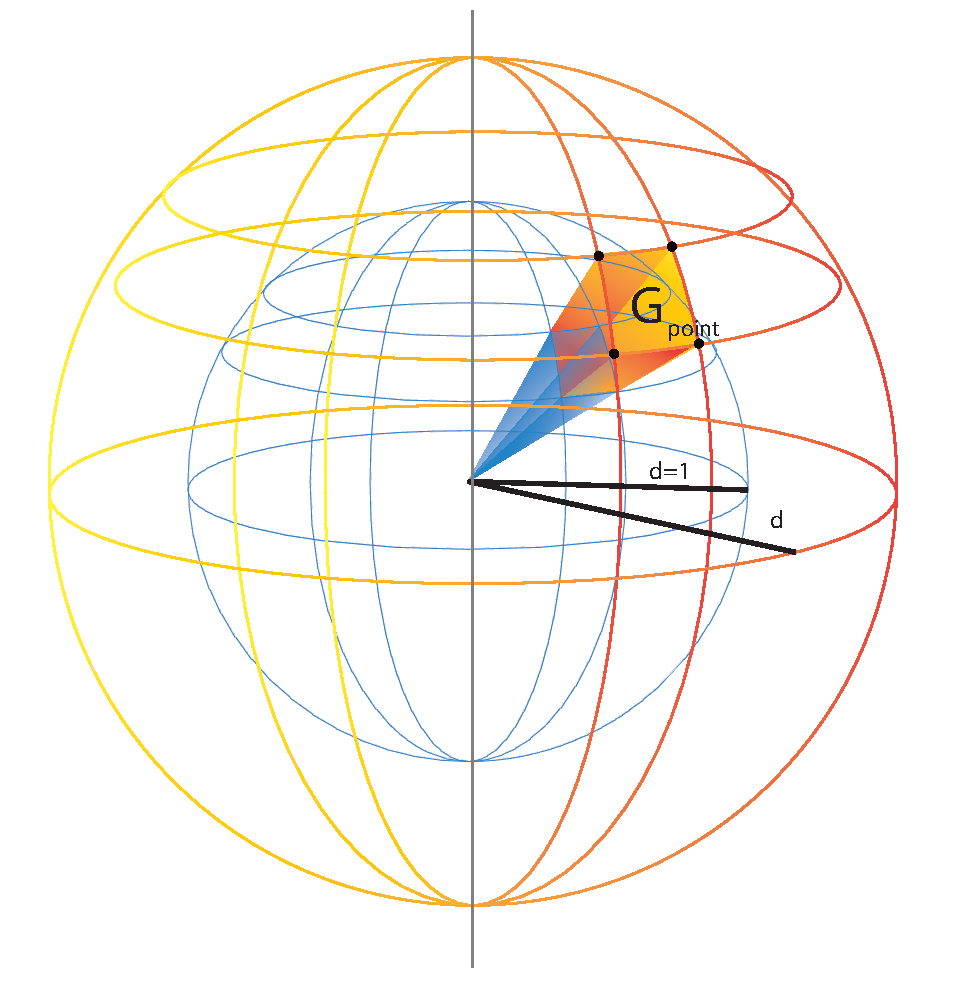
\includegraphics[width=0.6\textwidth, trim={0cm 0cm 0cm 0cm},clip]{illustrations/PointEmitter.pdf}}
%\subcaptionbox{$ 2r =\sqrt{2}L$  \label{xystion-simple-grid-ratio}}
\caption{The area of each grid cell $G$ expands as diameter increases. Back dots are lightlanes which convey photons from this point. Area of cell G increase exponentially with distance $d$ from a starting point of available lightlanes determined by $b$.}
\label{fig:pointEmitter1}
{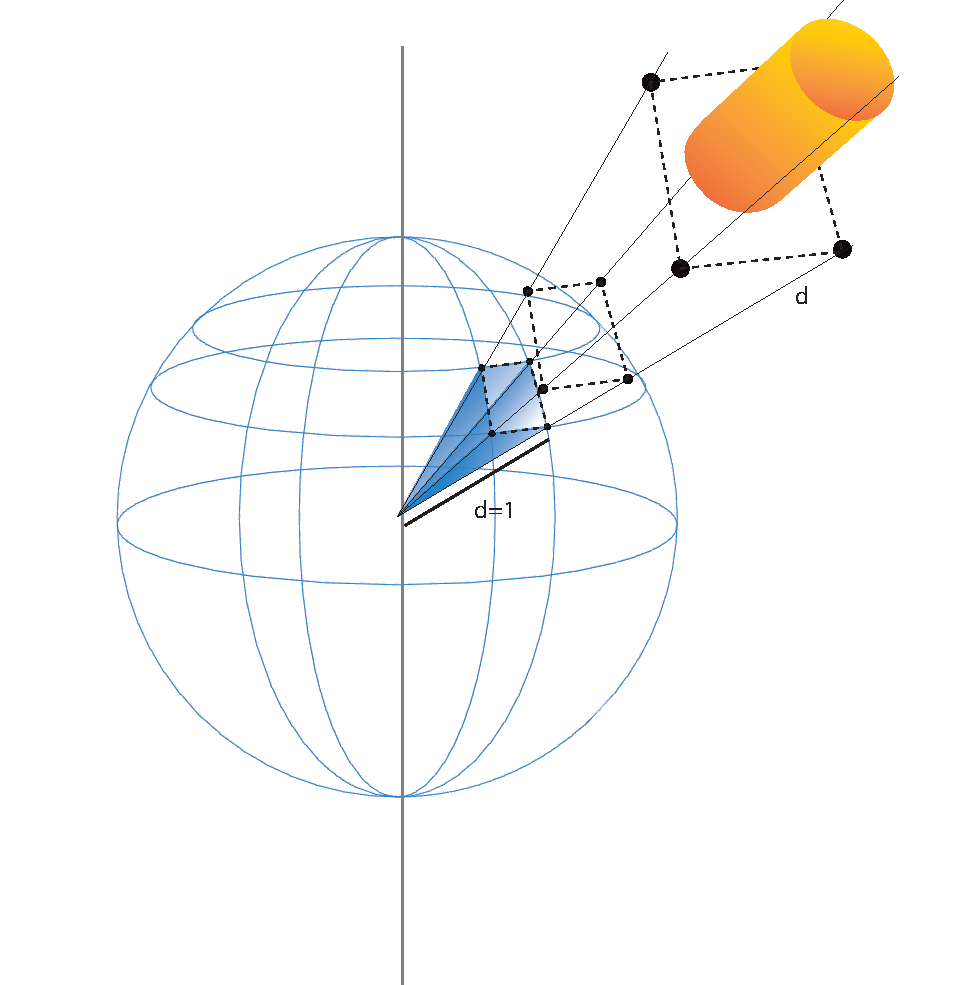
\includegraphics[width=0.6\textwidth, trim={0cm 0cm 0cm 0cm},clip]{illustrations/PointEmitter2.pdf}}
%\subcaptionbox{$ 2r =\sqrt{2}L$  \label{xystion-simple-grid-ratio}}
\caption{A detector, such as a telescope  (yellow cylinder), being stationary with respect to the emitter frame, can be positioned so that it is dark-zoned (not intersecting any lightlanes whatsoever), or Lucky Laned (intersecting exactly one lightlane all the time)}
\label{fig:pointEmitter2}
\end{figure}

